%!TEX root = ../presentation.tex
\section{Teamarbeit}

\subsection{Kommunikation}
\begin{frame}{Kommunikation}
    \begin{itemize}
        \item Kommunikation über Matrix (Element)
        \item Wöchentliche Treffen am Montag
        \item GitHub Issues
    \end{itemize}
\end{frame}

\subsection{Stufe 1}
\begin{frame}{Stufe 1}
    \begin{figure}
        \centering
        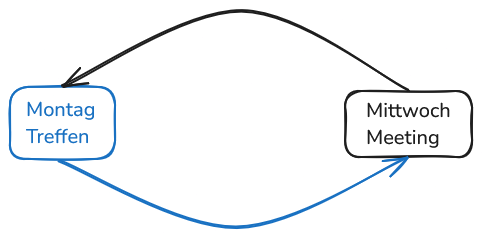
\includegraphics[width=0.6\linewidth]{pictures/level1}
        \label{fig:lvl1}
    \end{figure}
\end{frame}

\begin{frame}{Problem: Programmieren beim Montag Treffen}
\begin{figure}
    \centering
    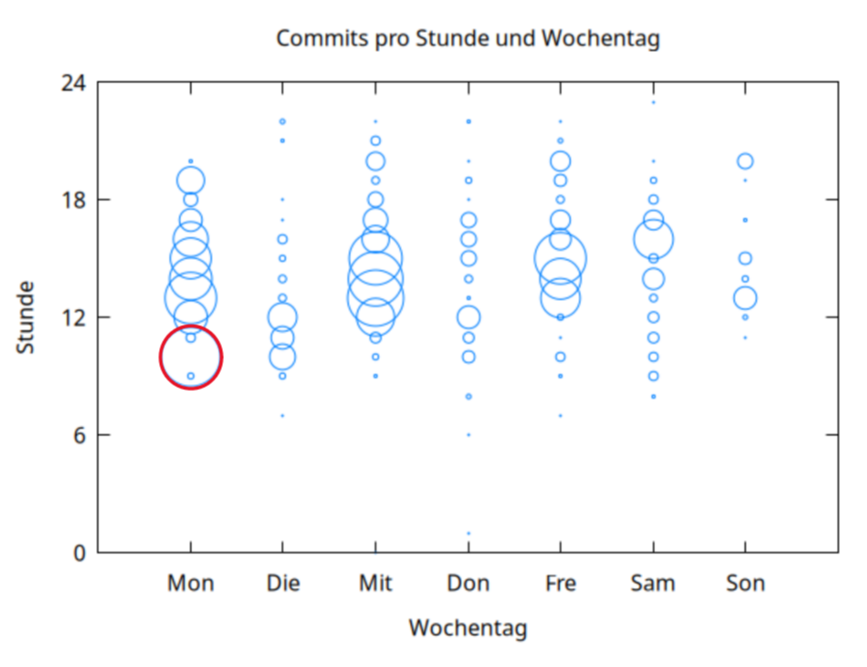
\includegraphics[width=0.52\linewidth]{pictures/hours}
    \label{fig:commit-hours}
\end{figure}
\end{frame}

\subsection{Stufe 2}
\begin{frame}{Stufe 2}
\begin{figure}
    \centering
    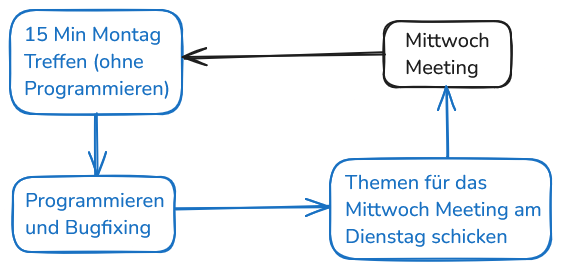
\includegraphics[width=0.6\linewidth]{pictures/level2}
    \label{fig:lvl2}
\end{figure}
\end{frame}

\subsection{Stufe 3}
\begin{frame}{Stufe 3}
\begin{figure}
    \centering
    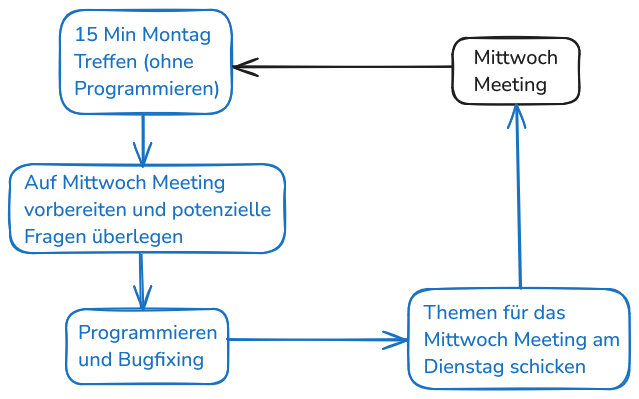
\includegraphics[width=0.6\linewidth]{pictures/level3}
    \label{fig:lvl3}
\end{figure}
\end{frame}